\chapter{Modeling}
\label{modeling}
This chapter lays out the mathematical framework used in the forthcoming design work. The model derived here 
is used to dictate simulation modeling as well as controller design. A brief overview of the platform's drivetrain and 
steering mechanisms is provided, before they are translated to a mathematical expression analytically.

Ultimately, a simplified model based on the bicycle kinematic model is derived, involving the golf cart's longitudinal dynamics
to model the relationship between motor torque and velocity.

\section{Mechanical Layout and Drivetrain}
\label{mech_layout}
%[Describe motor -> transaxle -> wheel and steer motor -> shaft -> encoder relationships]
The drivetrain of the golf cart consists of a permanent magnet alternating current (PMAC) motor connected to the 
original transaxle of the cart. This is accomplished by connecting the motor output to the transaxle input via a chain.
From this point, power is transferred to the rear wheels via the transaxle.

The steering system of the golf cart consists of a rack and pinion, controlled by a main steering column to which a 
DC motor is attached. This connection is mechanically achieved between the output shaft of the motor's gearbox and the 
steering column via a chain and sprocket. The steering column then actuates the steering rack as if the steering wheel
were being turned, according to the DC motor input. 

\begin{figure}[h]
  \centering
  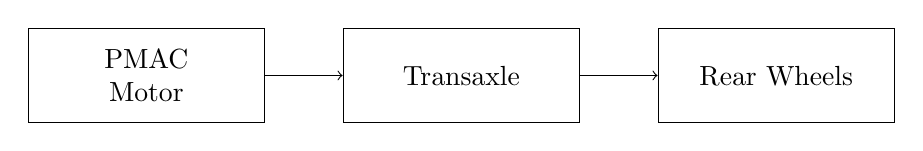
\begin{tikzpicture}[
    block/.style={draw, rectangle, minimum height=1.2cm, minimum width=3.0cm, align=center}
  ]

    % Blocks
    \node[block] at (0,0)    (motor)    {PMAC\\Motor};
    \node[block] at (4,0)    (transaxle){Transaxle};
    \node[block] at (8,0)    (wheels)   {Rear Wheels};

    % Simple connections (no arrows, no labels)
    \draw[->] (motor) -- (transaxle);
    \draw[->] (transaxle) -- (wheels);

  \end{tikzpicture}
  \caption{Mechanical Drivetrain Layout}
  \label{fig:drivetrain_layout}
\end{figure}

\begin{figure}[h]
  \centering
  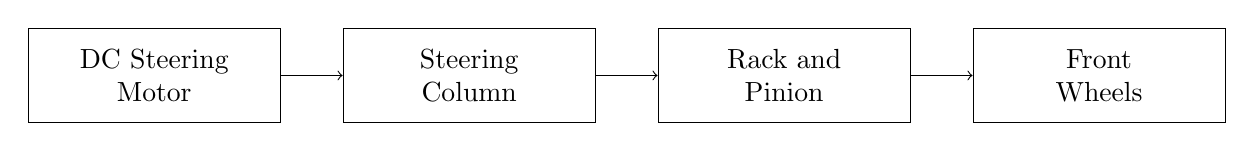
\begin{tikzpicture}[
    block/.style={draw, rectangle, minimum height=1.2cm, minimum width=3.2cm, align=center}
  ]
    % Blocks
    \node[block] at (0,0)    (motor)   {DC Steering\\Motor};
    \node[block] at (4,0)    (column)  {Steering\\Column};
    \node[block] at (8,0)   (rack)    {Rack and\\Pinion};
    \node[block] at (12,0)   (wheels)  {Front\\Wheels};

    % Simple connections (no arrows, no labels)
    \draw[->] (motor) -- (column);
    \draw[->] (column) -- (rack);
    \draw[->] (rack) -- (wheels);

  \end{tikzpicture}
  \caption{Steering System Layout}
  \label{fig:steering_layout}
\end{figure}

\section{Simplifications and Assumptions}
\label{simplifications_and_assumptions}
The essential idea of the mathematical model for the golf cart is to capture how motor torque relates to linear velocity,
and how steering angle changes relate to translation of the platform. The following constraints are imposed to make simulation modeling
and controller design more straightforward for this component of the project:

\subsection{Velocity Operating Region}
\label{speed_constraint}
Due to the low speed operating region of the golf cart (i.e.\ less than 20 mph), the effects of certain lateral dynamic forces, such as lateral tire slip,
are ignored. This simplification is based on Kong et al.\ \cite{kong2015}, whose work shows that below certain speeds and lateral forces, a simplified 
model is sufficient to describe platform motion. Additionally, a pure rolling model is assumed, where the tires do not slip in the longitudinal direction.

\subsection{Terrain Considerations}
\label{terrain_constraint}
For modeling purposes, terrain is presumed to be level enough such that the inclination or declination of the cart
does not meaningfully contribute to the sum of the longitudinal forces acting on the golf cart. Grade forces and load transfer dynamics are 
excluded from the model. Mathematically, this is represented as any force scaled by sin($\theta$) set to 0.

\subsection{Aerodynamics}
\label{air_constraint}
To simplify the modeling math, aerodynamic drag is neglected. At the low speed region the platform operates at, the aerodynamic drag should be small enough
to only cause a minor mismatch between simulation and reality. 

\subsection{Suspension Dynamics}
\label{suspension_constraint}
Due to the low velocity operating region and terrain assumptions, effects of suspension and pitch dynamics are neglected. It is assumed that the influence
these systems would have on the description and control of the vehicle are negligible.

\subsection{Drivetrain Dynamics}
\label{drivetrain_constraint}
The inertial effect of the drivetrain, such as motor and transaxle inertia, on longitudinal dynamics is neglected for now. Future work may explore experimental measuring of this value to improve
the fidelity of the model. However, the inertial effect of the wheel and hub rotation in the sense of effective mass is considered, and is included in the term $J_\text{eq}$.

\subsection{Physical Modeling}
\label{physics_constraint}
For modeling purposes, the cart is assumed to be a symmetric mass with a center of gravity in the geometric center of the body. The effect this has simplifies moments of inertia, and places 
the CoG equidistant from both axles of the platform.

\section{Longitudinal Dynamics}
\label{longitudinal_dynamics}
The longitudinal dynamics are the body frame forces exerted along the horizontal plane of the platform. These can be derived from Newton's second law, as presented in literature such as Rajamani \cite{rajamani}
and Gillespie \cite{gillespie}. Accounting for the assumptions and simplifications made when considering the modeling of the platform, the longitudinal dynamics are as follows:
    \vspace{10\baselineskip}
    \begin{figure}[htbp]
        \centering
        \begin{tikzpicture}
            % Parameters
            \def\R{1}          % wheel radius
            \def\yrear{1}      % wheel center height
            \def\xrear{7}      % rear wheel center x
            \def\xfront{3}     % front wheel center x

            % Ground
            \draw (0,0) -- (10,0);

            % Wheels
            \draw (\xrear,\yrear) circle (\R);
            \draw (\xfront,\yrear) circle (\R);

            % Cart body: bottom at top of wheels (y = yrear + R)
            \draw (2,\yrear+\R) rectangle (8,\yrear+\R+2);

        % ----- Center of mass and weight -----
            \coordinate (C) at (5,\yrear+\R+1);   % center of mass
            \fill (C) circle (1.5pt);
            \node[above] at (C) {$m_{\mathrm{eq}}$};% point label
            \draw[->] (C) -- ++(0,-1)
                node[below] {$m_{\mathrm{eq}} g$};% weight force
            % Velocity arrow (to the left)
            \draw[->] (2,\yrear+\R+0.5) -- (0.7,\yrear+\R+0.5)
                node[above,pos=0.6] {$v$};

            % Drive force from rear wheel, just above ground
            \draw[->] (\xrear-0.15,0.15) -- (\xrear-1.85,0.15)
                node[above,pos=0.8] {$F_\text{drive}$};

            % Brake force from front wheel, just above ground
            \draw[->] (\xrear+0.15,0.15) -- (\xrear+1.8,0.15)
                node[above,pos=0.8] {$F_\text{brake}$};

            % Rolling resistance at front wheel, slightly below ground
            \draw[->] (\xrear,-0.3) -- (\xrear+1.8,-0.3)
                node[below,pos=0.6] {$F_\text{roll}$};

        \end{tikzpicture}
        \caption{Diagram of Forces Acting on Platform along Longitudinal Axis}
        \label{fig:longitudinal-force-free-body}
    \end{figure}

    The above free body diagram is summarized in the following equation:
    %Longitudinal Dynamics Eqs
    %\setlength{\mathindent}{1cm}
    \begin{align}
        &m_\text{eq}\,\dot v = \sum F_x
        \label{eq:newton_long} \\[0.5em]
        \intertext{Where the sum of forces is:}
        &\sum F_x = F_\text{drive} - F_\text{brake} - F_\text{roll}
        \label{eq:force_sum} \\[0.5em]
        \intertext{And the individual forces are given by:}
        &F_\text{drive} = \frac{\eta_d \, i_\text{tot}}{r_w}\,T_\text{motor}
        \label{eq:f_drive_def} \\[0.5em]
        &F_\text{brake} = \frac{T_\text{brake}}{r_w}
        \label{eq:f_brake_def} \\[0.5em]
        &F_\text{roll} = C_{rr}\,m\,g
        \label{eq:f_roll_def} \\[0.5em]
        &m_\text{eq} = m + \frac{J_\text{eq}}{r_w^2}
        \label{eq:meq_def}
    \end{align}

\section{Lateral Kinematics}
\label{lateral_kinematics}
The lateral motion of the golf cart is modeled using a planar kinematic bicycle model. The goal of this model 
is to capture how changes in steering angle translate to motion of the cart in the world frame. As presented in 
Kong et al.\ \cite{kong2015}, this simplified representation is sufficient at low speeds and for the smooth 
maneuvers considered in this work.

A world–fixed frame $\{W\}$ with coordinates $(x, y)$ is defined, and a body-fixed frame $\{B\}$ is attached to 
the golf cart. The state of the lateral model is

\begin{equation}
    \begin{aligned}
        \mathbf{q} &= 
        \begin{bmatrix}
            x \\ y \\ \psi
        \end{bmatrix}
    \end{aligned}
    \label{eq:lateral_state}
\end{equation}

where $(x, y)$ is the position of a reference point on the cart, the center of the rear axle, expressed in 
$\{W\}$, and $\psi$ is the yaw heading of the cart with respect to $\{W\}$. The inputs to the kinematic model are
the longitudinal speed $v$ along the body $x$–axis and the front wheel steering angle $\delta$.
    \vspace{2\baselineskip}
    \begin{figure}[htbp]
        \centering
        \begin{tikzpicture}[
        scale=1.0,
        >=Stealth,
        line cap=round,
        line join=round,
        every node/.style={font=\small}
        ]

        % Parameters (drawing only)
        \def\psiang{30}   % vehicle heading angle [deg]
        \def\deltaang{15} % steering angle [deg]
        \def\betaang{25}  % slip angle [deg]
        \def\L{4.0}       % wheelbase in drawing units

        \pgfmathsetmacro{\psiplusdelta}{\psiang+\deltaang}
        \pgfmathsetmacro{\psiplusbeta}{\psiang+\betaang}

        % World frame axes
        \draw[->] (0,0) -- (8,0) node[below right] {$X_w$};
        \draw[->] (0,0) -- (0,6) node[above left] {$Y_w$};

        % Rear and front axle centres
        \coordinate (R) at (2,1.2);
        \coordinate (F) at ($(R)+(\psiang:\L)$);

        % Reference point (e.g. CG) between axles
        \coordinate (C) at ($(R)!0.45!(F)$);
        % Dot at CoM
        \fill (C) circle (1.5pt);
        % Dashed world-coordinate lines through C (x,y)
        \draw[densely dashed,thin] (0,0 |- C) -- ($(C)+(1.2,0)$);
        \node[left]  at (0,0 |- C) {$y$};

        \draw[densely dashed,thin] (0,0 -| C) -- (C);
        \node[below] at (0,0 -| C) {$x$};

        % Vehicle centreline (bicycle body)
        \draw[thick] (R) -- (F);

        % Rear wheel: aligned with body line
        \draw[thick] (R)
            ellipse[x radius=0.7, y radius=0.25, rotate=\psiang];

        % Front wheel: aligned with steered direction (psi + delta)
        \draw[thick] (F)
            ellipse[x radius=0.7, y radius=0.25, rotate=\psiplusdelta];
        % Reference rays at the front axle:
        % body x-axis
        \draw[thin] (F) -- ($(F)+(\psiang:1.2)$);
        % wheel axis (through the long end of the tire)
        \draw[thin] (F) -- ($(F)+(\psiplusdelta:1.2)$);

        % Dashed extension of body direction at front (reference for delta)
        \draw[densely dashed] (F) -- ($(F)+(\psiang:1.0)$);

        % Steering angle delta between body x-axis and wheel axis
        \draw[->] (F) ++(\psiang:0.8)
            arc[start angle=\psiang, end angle=\psiplusdelta, radius=0.8];
        \node[above right] at ($(F)+(\psiang+0.5*\deltaang:1.0)$) {$\delta$};

        % Longitudinal speed vector v_B at C with slip beta
        \draw[->,thick] (C) -- ($(C)+(\psiplusbeta:1.8)$)
            node[above] {$v$};

        % Yaw angle psi between world X and body, sitting on the y-dashed line
        \draw[->] (C) ++(0:1.0)
            arc[start angle=0, end angle=\psiang, radius=1.0];
        \node[right] at ($(C)+(0.5,0.2)$) {$\psi$};

        % Wheelbase L, between wheel centers, offset slightly normal to the body line
        \draw[<->]
        ($(R)+(\psiang-90:0.5)$) -- ($(F)+(\psiang-90:0.5)$)
        node[midway, below right] {$L$};

        % Instantaneous centre of rotation O
        \coordinate (O) at (1.0,5.0);
        \fill (O) circle (1pt);
        \node[above left] at (O) {$O$};

        % Dashed lines from O to both wheels and CG
        \draw[densely dashed,thin] (O) -- (R);
        \draw[densely dashed,thin] (O) -- (C) node[midway, above] {$R$};
        \draw[densely dashed,thin] (O) -- (F);

        \end{tikzpicture}
        \caption{Diagram of Bicycle Model}
        \label{fig:bicycle-model-free-body}
    \end{figure}

Here, O labels the instantaneous center of rotation, R is the radius of rotation, {$v$} is the linear velocity of the cart expressed in $\{W\}$. $L$ is the wheelbase of the platform, and ${\delta}$ is the 
steering angle expressed in $\{B\}$. Thus, the lateral motion is described by the standard kinematic bicycle equations
\begin{align}
    \dot{x} &= v \cos\psi, \label{eq:bicycle_xdot} \\[0.3em]
    \dot{y} &= v \sin\psi, \label{eq:bicycle_ydot} \\[0.3em]
    \dot{\psi} &= \frac{v}{L}\tan\delta, 
    \label{eq:bicycle_psidot}
\end{align}

\section{Combined Model}
\label{combined_model}
These two models combined represent the unified set of equations used to model the behavior of the platform. These equations will be used as a basis for designing the parameters of the simulation model, and 
for designing any necessary controllers. The equations are summarized as the state space model for the platform, and are provided in this section.

Combining the body frame representation \eqref{eq:lateral_state} of the platform with its expression for velocity from the longitudinal dynamics yields the following state vector to describe the motion of the 
platform with reference to world frame coordinates:

\begin{equation}
    \mathbf{x} =
    \begin{bmatrix}
        x \\[0.25em]
        y \\[0.25em]
        \psi \\[0.25em]
        v
    \end{bmatrix}
    \label{eq:combined_state_vector}
\end{equation}

The lateral motion is described by the kinematic bicycle model introduced in Section~\ref{lateral_kinematics}, with
\begin{align}
    \dot x &= v \cos\psi,
    \label{eq:combined_xdot} \\[0.5em]
    \dot y &= v \sin\psi,
    \label{eq:combined_ydot} \\[0.5em]
    \dot\psi &= \frac{v}{L}\,\tan\delta,
    \label{eq:combined_psidot}
\end{align}
where \(L\) is the wheelbase and \(\delta\) is the front wheel steering angle.

The longitudinal dynamics are given by the force balance developed in Section~\ref{longitudinal_dynamics}. Recalling Newton’s law in \eqref{eq:newton_long} with the longitudinal force decomposition
in \eqref{eq:force_sum}, the linear acceleration can be described as
\begin{equation}
    \dot v = \frac{1}{m_\text{eq}}\bigl(F_\text{drive} - F_\text{brake} - F_\text{roll}\bigr),
    \label{eq:combined_vdot_generic}
\end{equation}
where the effective mass \(m_\text{eq}\) and the individual force terms are defined in \eqref{eq:f_drive_def}–\eqref{eq:f_roll_def}.

For later controller design it is convenient to identify the actuator inputs that enter these equations. The motor torque \(T_\text{motor}\) and brake torque \(T_\text{brake}\) determine the drive
and brake forces through \eqref{eq:f_drive_def} and \eqref{eq:f_brake_def}, while the steering angle \(\delta\) appears in the bicycle kinematics in \eqref{eq:combined_psidot}. These three control signals
can be organized into the following control vector $u$ as
\begin{equation}
    \mathbf{u} =
    \begin{bmatrix}
        T_\text{motor} \\[0.25em]
        T_\text{brake} \\[0.25em]
        \delta
    \end{bmatrix}
    \label{eq:combined_input_vector}
\end{equation}

Using the relationships defined in \eqref{eq:combined_xdot}–\eqref{eq:combined_vdot_generic}, the combined planar model can be expressed in nonlinear state space form as
\begin{equation}
    \dot{\mathbf{x}} = \mathbf{f}(\mathbf{x},\mathbf{u}) =
    \begin{bmatrix}
        v \cos\psi \\[0.25em]
        v \sin\psi \\[0.25em]
        \dfrac{v}{L}\,\tan\delta \\[0.75em]
        \dfrac{\eta_d i_{\text{tot}}}{m_{\text{eq}} r_w}\,T_\text{motor}
        - \dfrac{1}{m_{\text{eq}} r_w}\,T_{\text{brake}}
        - \dfrac{C_{rr} m g}{m_{\text{eq}}}
    \end{bmatrix}.
    \label{eq:combined_state_space_expanded}
\end{equation}


